\documentclass[1p]{elsarticle_modified}
%\bibliographystyle{elsarticle-num}

%\usepackage[colorlinks]{hyperref}
%\usepackage{abbrmath_seonhwa} %\Abb, \Ascr, \Acal ,\Abf, \Afrak
\usepackage{amsfonts}
\usepackage{amssymb}
\usepackage{amsmath}
\usepackage{amsthm}
\usepackage{scalefnt}
\usepackage{amsbsy}
\usepackage{kotex}
\usepackage{caption}
\usepackage{subfig}
\usepackage{color}
\usepackage{graphicx}
\usepackage{xcolor} %% white, black, red, green, blue, cyan, magenta, yellow
\usepackage{float}
\usepackage{setspace}
\usepackage{hyperref}

\usepackage{tikz}
\usetikzlibrary{arrows}

\usepackage{multirow}
\usepackage{array} % fixed length table
\usepackage{hhline}

%%%%%%%%%%%%%%%%%%%%%
\makeatletter
\renewcommand*\env@matrix[1][\arraystretch]{%
	\edef\arraystretch{#1}%
	\hskip -\arraycolsep
	\let\@ifnextchar\new@ifnextchar
	\array{*\c@MaxMatrixCols c}}
\makeatother %https://tex.stackexchange.com/questions/14071/how-can-i-increase-the-line-spacing-in-a-matrix
%%%%%%%%%%%%%%%

\usepackage[normalem]{ulem}

\newcommand{\msout}[1]{\ifmmode\text{\sout{\ensuremath{#1}}}\else\sout{#1}\fi}
%SOURCE: \msout is \stkout macro in https://tex.stackexchange.com/questions/20609/strikeout-in-math-mode

\newcommand{\cancel}[1]{
	\ifmmode
	{\color{red}\msout{#1}}
	\else
	{\color{red}\sout{#1}}
	\fi
}

\newcommand{\add}[1]{
	{\color{blue}\uwave{#1}}
}

\newcommand{\replace}[2]{
	\ifmmode
	{\color{red}\msout{#1}}{\color{blue}\uwave{#2}}
	\else
	{\color{red}\sout{#1}}{\color{blue}\uwave{#2}}
	\fi
}

\newcommand{\Sol}{\mathcal{S}} %segment
\newcommand{\D}{D} %diagram
\newcommand{\A}{\mathcal{A}} %arc


%%%%%%%%%%%%%%%%%%%%%%%%%%%%%5 test

\def\sl{\operatorname{\textup{SL}}(2,\Cbb)}
\def\psl{\operatorname{\textup{PSL}}(2,\Cbb)}
\def\quan{\mkern 1mu \triangleright \mkern 1mu}

\theoremstyle{definition}
\newtheorem{thm}{Theorem}[section]
\newtheorem{prop}[thm]{Proposition}
\newtheorem{lem}[thm]{Lemma}
\newtheorem{ques}[thm]{Question}
\newtheorem{cor}[thm]{Corollary}
\newtheorem{defn}[thm]{Definition}
\newtheorem{exam}[thm]{Example}
\newtheorem{rmk}[thm]{Remark}
\newtheorem{alg}[thm]{Algorithm}

\newcommand{\I}{\sqrt{-1}}
\begin{document}

%\begin{frontmatter}
%
%\title{Boundary parabolic representations of knots up to 8 crossings}
%
%%% Group authors per affiliation:
%\author{Yunhi Cho} 
%\address{Department of Mathematics, University of Seoul, Seoul, Korea}
%\ead{yhcho@uos.ac.kr}
%
%
%\author{Seonhwa Kim} %\fnref{s_kim}}
%\address{Center for Geometry and Physics, Institute for Basic Science, Pohang, 37673, Korea}
%\ead{ryeona17@ibs.re.kr}
%
%\author{Hyuk Kim}
%\address{Department of Mathematical Sciences, Seoul National University, Seoul 08826, Korea}
%\ead{hyukkim@snu.ac.kr}
%
%\author{Seokbeom Yoon}
%\address{Department of Mathematical Sciences, Seoul National University, Seoul, 08826,  Korea}
%\ead{sbyoon15@snu.ac.kr}
%
%\begin{abstract}
%We find all boundary parabolic representation of knots up to 8 crossings.
%
%\end{abstract}
%\begin{keyword}
%    \MSC[2010] 57M25 
%\end{keyword}
%
%\end{frontmatter}

%\linenumbers
%\tableofcontents
%
\newcommand\colored[1]{\textcolor{white}{\rule[-0.35ex]{0.8em}{1.4ex}}\kern-0.8em\color{red} #1}%
%\newcommand\colored[1]{\textcolor{white}{ #1}\kern-2.17ex	\textcolor{white}{ #1}\kern-1.81ex	\textcolor{white}{ #1}\kern-2.15ex\color{red}#1	}

{\Large $\underline{12a_{0211}~(K12a_{0211})}$}

\setlength{\tabcolsep}{10pt}
\renewcommand{\arraystretch}{1.6}
\vspace{1cm}\begin{tabular}{m{100pt}>{\centering\arraybackslash}m{274pt}}
\multirow{5}{120pt}{
	\centering
	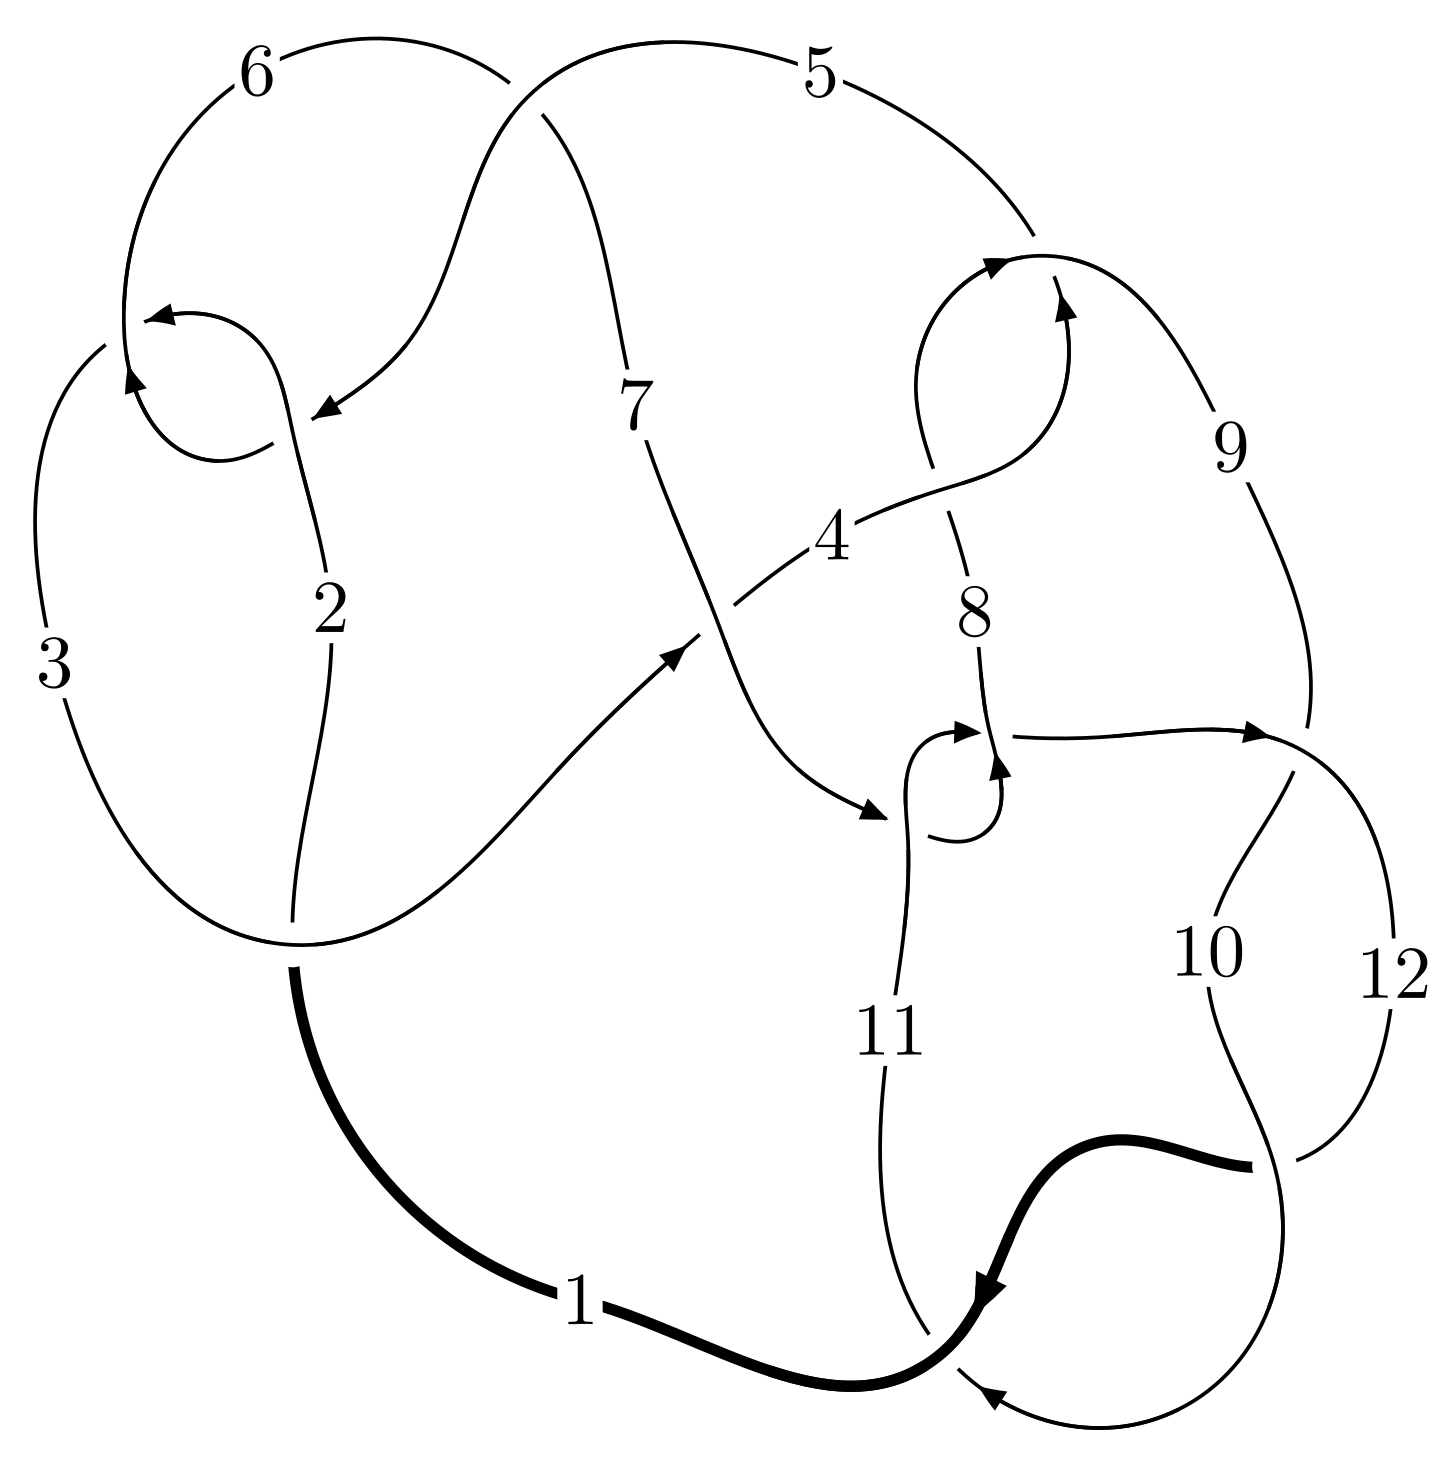
\includegraphics[width=112pt]{../../../GIT/diagram.site/Diagrams/png/1012_12a_0211.png}\\
\ \ \ A knot diagram\footnotemark}&
\allowdisplaybreaks
\textbf{Linearized knot diagam} \\
\cline{2-2}
 &
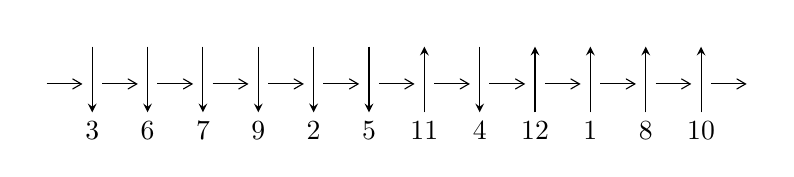
\begin{tikzpicture}[x=20pt, y=17pt]
	% nodes
	\node (C0) at (0, 0) {};
	\node (C1) at (1, 0) {};
	\node (C1U) at (1, +1) {};
	\node (C1D) at (1, -1) {3};

	\node (C2) at (2, 0) {};
	\node (C2U) at (2, +1) {};
	\node (C2D) at (2, -1) {6};

	\node (C3) at (3, 0) {};
	\node (C3U) at (3, +1) {};
	\node (C3D) at (3, -1) {7};

	\node (C4) at (4, 0) {};
	\node (C4U) at (4, +1) {};
	\node (C4D) at (4, -1) {9};

	\node (C5) at (5, 0) {};
	\node (C5U) at (5, +1) {};
	\node (C5D) at (5, -1) {2};

	\node (C6) at (6, 0) {};
	\node (C6U) at (6, +1) {};
	\node (C6D) at (6, -1) {5};

	\node (C7) at (7, 0) {};
	\node (C7U) at (7, +1) {};
	\node (C7D) at (7, -1) {11};

	\node (C8) at (8, 0) {};
	\node (C8U) at (8, +1) {};
	\node (C8D) at (8, -1) {4};

	\node (C9) at (9, 0) {};
	\node (C9U) at (9, +1) {};
	\node (C9D) at (9, -1) {12};

	\node (C10) at (10, 0) {};
	\node (C10U) at (10, +1) {};
	\node (C10D) at (10, -1) {1};

	\node (C11) at (11, 0) {};
	\node (C11U) at (11, +1) {};
	\node (C11D) at (11, -1) {8};

	\node (C12) at (12, 0) {};
	\node (C12U) at (12, +1) {};
	\node (C12D) at (12, -1) {10};
	\node (C13) at (13, 0) {};

	% arrows
	\draw[->,>={angle 60}]
	(C0) edge (C1) (C1) edge (C2) (C2) edge (C3) (C3) edge (C4) (C4) edge (C5) (C5) edge (C6) (C6) edge (C7) (C7) edge (C8) (C8) edge (C9) (C9) edge (C10) (C10) edge (C11) (C11) edge (C12) (C12) edge (C13) ;	\draw[->,>=stealth]
	(C1U) edge (C1D) (C2U) edge (C2D) (C3U) edge (C3D) (C4U) edge (C4D) (C5U) edge (C5D) (C6U) edge (C6D) (C7D) edge (C7U) (C8U) edge (C8D) (C9D) edge (C9U) (C10D) edge (C10U) (C11D) edge (C11U) (C12D) edge (C12U) ;
	\end{tikzpicture} \\
\hhline{~~} \\& 
\textbf{Solving Sequence} \\ \cline{2-2} 
 &
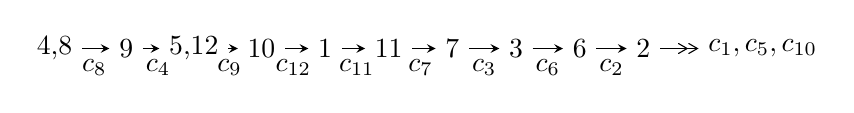
\begin{tikzpicture}[x=23pt, y=7pt]
	% node
	\node (A0) at (-1/8, 0) {4,8};
	\node (A1) at (1, 0) {9};
	\node (A2) at (33/16, 0) {5,12};
	\node (A3) at (25/8, 0) {10};
	\node (A4) at (33/8, 0) {1};
	\node (A5) at (41/8, 0) {11};
	\node (A6) at (49/8, 0) {7};
	\node (A7) at (57/8, 0) {3};
	\node (A8) at (65/8, 0) {6};
	\node (A9) at (73/8, 0) {2};
	\node (C1) at (1/2, -1) {$c_{8}$};
	\node (C2) at (3/2, -1) {$c_{4}$};
	\node (C3) at (21/8, -1) {$c_{9}$};
	\node (C4) at (29/8, -1) {$c_{12}$};
	\node (C5) at (37/8, -1) {$c_{11}$};
	\node (C6) at (45/8, -1) {$c_{7}$};
	\node (C7) at (53/8, -1) {$c_{3}$};
	\node (C8) at (61/8, -1) {$c_{6}$};
	\node (C9) at (69/8, -1) {$c_{2}$};
	\node (A10) at (11, 0) {$c_{1},c_{5},c_{10}$};

	% edge
	\draw[->,>=stealth]	
	(A0) edge (A1) (A1) edge (A2) (A2) edge (A3) (A3) edge (A4) (A4) edge (A5) (A5) edge (A6) (A6) edge (A7) (A7) edge (A8) (A8) edge (A9) ;
	\draw[->>,>={angle 60}]	
	(A9) edge (A10);
\end{tikzpicture} \\ 

\end{tabular} \\

\footnotetext{
The image of knot diagram is generated by the software ``\textbf{Draw programme}" developed by Andrew Bartholomew(\url{http://www.layer8.co.uk/maths/draw/index.htm\#Running-draw}), where we modified some parts for our purpose(\url{https://github.com/CATsTAILs/LinksPainter}).
}\phantom \\ \newline 
\centering \textbf{Ideals for irreducible components\footnotemark of $X_{\text{par}}$} 
 
\begin{align*}
I^u_{1}&=\langle 
-9.86194\times10^{263} u^{97}+1.50956\times10^{264} u^{96}+\cdots+4.00373\times10^{264} b+1.42422\times10^{266},\\
\phantom{I^u_{1}}&\phantom{= \langle  }1.21954\times10^{264} u^{97}-1.97917\times10^{264} u^{96}+\cdots+8.00746\times10^{264} a-1.99719\times10^{266},\\
\phantom{I^u_{1}}&\phantom{= \langle  }u^{98}-2 u^{97}+\cdots-160 u+64\rangle \\
I^u_{2}&=\langle 
b,\;2 u^7-3 u^6-5 u^5+7 u^4+4 u^3-3 u^2+a-4,\;u^8- u^7-3 u^6+2 u^5+3 u^4-2 u-1\rangle \\
\\
I^v_{1}&=\langle 
a,\;26 v^5-33 v^4+317 v^3-123 v^2+413 b+89 v-685,\;v^6-3 v^5+15 v^4-24 v^3+11 v^2-6 v+1\rangle \\
\end{align*}
\raggedright * 3 irreducible components of $\dim_{\mathbb{C}}=0$, with total 112 representations.\\
\footnotetext{All coefficients of polynomials are rational numbers. But the coefficients are sometimes approximated in decimal forms when there is not enough margin.}
\newpage
\renewcommand{\arraystretch}{1}
\centering \section*{I. $I^u_{1}= \langle -9.86\times10^{263} u^{97}+1.51\times10^{264} u^{96}+\cdots+4.00\times10^{264} b+1.42\times10^{266},\;1.22\times10^{264} u^{97}-1.98\times10^{264} u^{96}+\cdots+8.01\times10^{264} a-2.00\times10^{266},\;u^{98}-2 u^{97}+\cdots-160 u+64 \rangle$}
\flushleft \textbf{(i) Arc colorings}\\
\begin{tabular}{m{7pt} m{180pt} m{7pt} m{180pt} }
\flushright $a_{4}=$&$\begin{pmatrix}0\\u\end{pmatrix}$ \\
\flushright $a_{8}=$&$\begin{pmatrix}1\\0\end{pmatrix}$ \\
\flushright $a_{9}=$&$\begin{pmatrix}1\\u^2\end{pmatrix}$ \\
\flushright $a_{5}=$&$\begin{pmatrix}- u\\- u^3+u\end{pmatrix}$ \\
\flushright $a_{12}=$&$\begin{pmatrix}-0.152300 u^{97}+0.247165 u^{96}+\cdots-4.59357 u+24.9416\\0.246319 u^{97}-0.377039 u^{96}+\cdots+7.83550 u-35.5724\end{pmatrix}$ \\
\flushright $a_{10}=$&$\begin{pmatrix}-0.0398059 u^{97}+0.0702429 u^{96}+\cdots-3.05431 u+8.48553\\-0.411031 u^{97}+0.653363 u^{96}+\cdots-7.40277 u+62.7622\end{pmatrix}$ \\
\flushright $a_{1}=$&$\begin{pmatrix}0.00297584 u^{97}-0.00863836 u^{96}+\cdots+1.05873 u-0.848853\\-0.411031 u^{97}+0.653363 u^{96}+\cdots-7.40277 u+62.7622\end{pmatrix}$ \\
\flushright $a_{11}=$&$\begin{pmatrix}-0.398619 u^{97}+0.624205 u^{96}+\cdots-12.4291 u+60.5140\\0.246319 u^{97}-0.377039 u^{96}+\cdots+7.83550 u-35.5724\end{pmatrix}$ \\
\flushright $a_{7}=$&$\begin{pmatrix}-0.402842 u^{97}+0.642002 u^{96}+\cdots-5.72372 u+61.7414\\0.405818 u^{97}-0.650640 u^{96}+\cdots+6.78245 u-62.5902\end{pmatrix}$ \\
\flushright $a_{3}=$&$\begin{pmatrix}0.0603712 u^{97}-0.0945033 u^{96}+\cdots+3.51045 u-8.93865\\-0.286712 u^{97}+0.446756 u^{96}+\cdots-6.09763 u+42.5150\end{pmatrix}$ \\
\flushright $a_{6}=$&$\begin{pmatrix}-0.402533 u^{97}+0.632225 u^{96}+\cdots-6.75744 u+60.4412\\0.389959 u^{97}-0.628287 u^{96}+\cdots+6.33110 u-60.7040\end{pmatrix}$ \\
\flushright $a_{2}=$&$\begin{pmatrix}0.0840663 u^{97}-0.138202 u^{96}+\cdots+6.02197 u-11.8518\\-0.634821 u^{97}+0.986175 u^{96}+\cdots-17.0563 u+92.8076\end{pmatrix}$\\&\end{tabular}
\flushleft \textbf{(ii) Obstruction class $= -1$}\\~\\
\flushleft \textbf{(iii) Cusp Shapes $= -1.75154 u^{97}+2.69397 u^{96}+\cdots-90.1293 u+259.318$}\\~\\
\newpage\renewcommand{\arraystretch}{1}
\flushleft \textbf{(iv) u-Polynomials at the component}\newline \\
\begin{tabular}{m{50pt}|m{274pt}}
Crossings & \hspace{64pt}u-Polynomials at each crossing \\
\hline $$\begin{aligned}c_{1},c_{6}\end{aligned}$$&$\begin{aligned}
&u^{98}+32 u^{97}+\cdots+46 u+1
\end{aligned}$\\
\hline $$\begin{aligned}c_{2},c_{5}\end{aligned}$$&$\begin{aligned}
&u^{98}+4 u^{97}+\cdots+14 u+1
\end{aligned}$\\
\hline $$\begin{aligned}c_{3}\end{aligned}$$&$\begin{aligned}
&u^{98}-4 u^{97}+\cdots+19016 u+4129
\end{aligned}$\\
\hline $$\begin{aligned}c_{4},c_{8}\end{aligned}$$&$\begin{aligned}
&u^{98}+2 u^{97}+\cdots+160 u+64
\end{aligned}$\\
\hline $$\begin{aligned}c_{7},c_{11}\end{aligned}$$&$\begin{aligned}
&u^{98}-4 u^{97}+\cdots-128 u+256
\end{aligned}$\\
\hline $$\begin{aligned}c_{9},c_{10},c_{12}\end{aligned}$$&$\begin{aligned}
&u^{98}+12 u^{97}+\cdots-31 u+1
\end{aligned}$\\
\hline
\end{tabular}\\~\\
\newpage\renewcommand{\arraystretch}{1}
\flushleft \textbf{(v) Riley Polynomials at the component}\newline \\
\begin{tabular}{m{50pt}|m{274pt}}
Crossings & \hspace{64pt}Riley Polynomials at each crossing \\
\hline $$\begin{aligned}c_{1},c_{6}\end{aligned}$$&$\begin{aligned}
&y^{98}+72 y^{97}+\cdots-2334 y+1
\end{aligned}$\\
\hline $$\begin{aligned}c_{2},c_{5}\end{aligned}$$&$\begin{aligned}
&y^{98}-32 y^{97}+\cdots-46 y+1
\end{aligned}$\\
\hline $$\begin{aligned}c_{3}\end{aligned}$$&$\begin{aligned}
&y^{98}+76 y^{96}+\cdots-284998790 y+17048641
\end{aligned}$\\
\hline $$\begin{aligned}c_{4},c_{8}\end{aligned}$$&$\begin{aligned}
&y^{98}-42 y^{97}+\cdots-87040 y+4096
\end{aligned}$\\
\hline $$\begin{aligned}c_{7},c_{11}\end{aligned}$$&$\begin{aligned}
&y^{98}-60 y^{97}+\cdots-3457024 y+65536
\end{aligned}$\\
\hline $$\begin{aligned}c_{9},c_{10},c_{12}\end{aligned}$$&$\begin{aligned}
&y^{98}-96 y^{97}+\cdots-903 y+1
\end{aligned}$\\
\hline
\end{tabular}\\~\\
\newpage\flushleft \textbf{(vi) Complex Volumes and Cusp Shapes}
$$\begin{array}{c|c|c}  
\text{Solutions to }I^u_{1}& \I (\text{vol} + \sqrt{-1}CS) & \text{Cusp shape}\\
 \hline 
\begin{aligned}
u &= \phantom{-}0.836034 + 0.535484 I \\
a &= -0.62066 - 1.46991 I \\
b &= -0.276978 - 1.030340 I\end{aligned}
 & \phantom{-}2.71965 - 2.17187 I & \phantom{-0.000000 } 0 \\ \hline\begin{aligned}
u &= \phantom{-}0.836034 - 0.535484 I \\
a &= -0.62066 + 1.46991 I \\
b &= -0.276978 + 1.030340 I\end{aligned}
 & \phantom{-}2.71965 + 2.17187 I & \phantom{-0.000000 } 0 \\ \hline\begin{aligned}
u &= \phantom{-}1.007890 + 0.057843 I \\
a &= \phantom{-}0.515193 + 1.015350 I \\
b &= \phantom{-}0.482660 + 0.606015 I\end{aligned}
 & -1.69730 - 0.04707 I & \phantom{-0.000000 } 0 \\ \hline\begin{aligned}
u &= \phantom{-}1.007890 - 0.057843 I \\
a &= \phantom{-}0.515193 - 1.015350 I \\
b &= \phantom{-}0.482660 - 0.606015 I\end{aligned}
 & -1.69730 + 0.04707 I & \phantom{-0.000000 } 0 \\ \hline\begin{aligned}
u &= \phantom{-}0.988943 + 0.038650 I \\
a &= \phantom{-}0.298767 + 1.109500 I \\
b &= -0.915779 + 0.645889 I\end{aligned}
 & \phantom{-}0.81536 + 3.65505 I & \phantom{-0.000000 } 0 \\ \hline\begin{aligned}
u &= \phantom{-}0.988943 - 0.038650 I \\
a &= \phantom{-}0.298767 - 1.109500 I \\
b &= -0.915779 - 0.645889 I\end{aligned}
 & \phantom{-}0.81536 - 3.65505 I & \phantom{-0.000000 } 0 \\ \hline\begin{aligned}
u &= \phantom{-}0.640994 + 0.748545 I \\
a &= -1.24753 - 1.31283 I \\
b &= \phantom{-}0.099282 - 1.047820 I\end{aligned}
 & \phantom{-}6.60141 - 1.31084 I & \phantom{-0.000000 } 0 \\ \hline\begin{aligned}
u &= \phantom{-}0.640994 - 0.748545 I \\
a &= -1.24753 + 1.31283 I \\
b &= \phantom{-}0.099282 + 1.047820 I\end{aligned}
 & \phantom{-}6.60141 + 1.31084 I & \phantom{-0.000000 } 0 \\ \hline\begin{aligned}
u &= \phantom{-}0.958058 + 0.352709 I \\
a &= \phantom{-}0.462382 + 0.808485 I \\
b &= -1.122110 + 0.350042 I\end{aligned}
 & -1.92679 - 1.50494 I & \phantom{-0.000000 } 0 \\ \hline\begin{aligned}
u &= \phantom{-}0.958058 - 0.352709 I \\
a &= \phantom{-}0.462382 - 0.808485 I \\
b &= -1.122110 - 0.350042 I\end{aligned}
 & -1.92679 + 1.50494 I & \phantom{-0.000000 } 0\\
 \hline 
 \end{array}$$\newpage$$\begin{array}{c|c|c}  
\text{Solutions to }I^u_{1}& \I (\text{vol} + \sqrt{-1}CS) & \text{Cusp shape}\\
 \hline 
\begin{aligned}
u &= -0.945192 + 0.184243 I \\
a &= \phantom{-}0.063153 + 1.354140 I \\
b &= -0.690539 + 0.806870 I\end{aligned}
 & \phantom{-}1.09894 - 0.93181 I & \phantom{-0.000000 } 0 \\ \hline\begin{aligned}
u &= -0.945192 - 0.184243 I \\
a &= \phantom{-}0.063153 - 1.354140 I \\
b &= -0.690539 - 0.806870 I\end{aligned}
 & \phantom{-}1.09894 + 0.93181 I & \phantom{-0.000000 } 0 \\ \hline\begin{aligned}
u &= -0.566049 + 0.872784 I \\
a &= \phantom{-}0.561625 - 0.370323 I \\
b &= -1.047790 + 0.313579 I\end{aligned}
 & \phantom{-}4.33302 - 0.85349 I & \phantom{-0.000000 } 0 \\ \hline\begin{aligned}
u &= -0.566049 - 0.872784 I \\
a &= \phantom{-}0.561625 + 0.370323 I \\
b &= -1.047790 - 0.313579 I\end{aligned}
 & \phantom{-}4.33302 + 0.85349 I & \phantom{-0.000000 } 0 \\ \hline\begin{aligned}
u &= -0.577362 + 0.766403 I \\
a &= -1.41361 + 1.28993 I \\
b &= \phantom{-}0.174263 + 1.005380 I\end{aligned}
 & \phantom{-}6.01938 - 4.43105 I & \phantom{-0.000000 } 0 \\ \hline\begin{aligned}
u &= -0.577362 - 0.766403 I \\
a &= -1.41361 - 1.28993 I \\
b &= \phantom{-}0.174263 - 1.005380 I\end{aligned}
 & \phantom{-}6.01938 + 4.43105 I & \phantom{-0.000000 } 0 \\ \hline\begin{aligned}
u &= -0.413184 + 0.978752 I \\
a &= \phantom{-}0.192652 - 0.001510 I \\
b &= \phantom{-}1.327370 - 0.296247 I\end{aligned}
 & \phantom{-}8.16464 - 2.11391 I & \phantom{-0.000000 } 0 \\ \hline\begin{aligned}
u &= -0.413184 - 0.978752 I \\
a &= \phantom{-}0.192652 + 0.001510 I \\
b &= \phantom{-}1.327370 + 0.296247 I\end{aligned}
 & \phantom{-}8.16464 + 2.11391 I & \phantom{-0.000000 } 0 \\ \hline\begin{aligned}
u &= \phantom{-}0.523046 + 0.927802 I \\
a &= \phantom{-}0.550866 + 0.336203 I \\
b &= -1.026850 - 0.381970 I\end{aligned}
 & \phantom{-}3.59665 + 6.49124 I & \phantom{-0.000000 } 0 \\ \hline\begin{aligned}
u &= \phantom{-}0.523046 - 0.927802 I \\
a &= \phantom{-}0.550866 - 0.336203 I \\
b &= -1.026850 + 0.381970 I\end{aligned}
 & \phantom{-}3.59665 - 6.49124 I & \phantom{-0.000000 } 0\\
 \hline 
 \end{array}$$\newpage$$\begin{array}{c|c|c}  
\text{Solutions to }I^u_{1}& \I (\text{vol} + \sqrt{-1}CS) & \text{Cusp shape}\\
 \hline 
\begin{aligned}
u &= -0.945040 + 0.577805 I \\
a &= \phantom{-}0.464812 - 0.635543 I \\
b &= -1.252900 - 0.141177 I\end{aligned}
 & \phantom{-}3.98973 + 1.09003 I & \phantom{-0.000000 } 0 \\ \hline\begin{aligned}
u &= -0.945040 - 0.577805 I \\
a &= \phantom{-}0.464812 + 0.635543 I \\
b &= -1.252900 + 0.141177 I\end{aligned}
 & \phantom{-}3.98973 - 1.09003 I & \phantom{-0.000000 } 0 \\ \hline\begin{aligned}
u &= -0.685394 + 0.556168 I \\
a &= -0.51862 + 2.07030 I \\
b &= \phantom{-}0.966579 + 0.148747 I\end{aligned}
 & \phantom{-}4.79276 + 3.49348 I & \phantom{-0.000000 } 0. - 7.89856 I \\ \hline\begin{aligned}
u &= -0.685394 - 0.556168 I \\
a &= -0.51862 - 2.07030 I \\
b &= \phantom{-}0.966579 - 0.148747 I\end{aligned}
 & \phantom{-}4.79276 - 3.49348 I & \phantom{-0.000000 -}0. + 7.89856 I \\ \hline\begin{aligned}
u &= \phantom{-}0.295338 + 0.821202 I \\
a &= \phantom{-}0.653295 + 0.245041 I \\
b &= -0.779521 - 0.351251 I\end{aligned}
 & -1.36442 + 1.59603 I & -6.13954 - 4.68221 I \\ \hline\begin{aligned}
u &= \phantom{-}0.295338 - 0.821202 I \\
a &= \phantom{-}0.653295 - 0.245041 I \\
b &= -0.779521 + 0.351251 I\end{aligned}
 & -1.36442 - 1.59603 I & -6.13954 + 4.68221 I \\ \hline\begin{aligned}
u &= \phantom{-}1.072730 + 0.347020 I \\
a &= \phantom{-}0.084885 - 1.334090 I \\
b &= \phantom{-}0.898101 - 0.581765 I\end{aligned}
 & -2.07276 - 0.59423 I & \phantom{-0.000000 } 0 \\ \hline\begin{aligned}
u &= \phantom{-}1.072730 - 0.347020 I \\
a &= \phantom{-}0.084885 + 1.334090 I \\
b &= \phantom{-}0.898101 + 0.581765 I\end{aligned}
 & -2.07276 + 0.59423 I & \phantom{-0.000000 } 0 \\ \hline\begin{aligned}
u &= -1.009660 + 0.504740 I \\
a &= -0.429556 + 1.236740 I \\
b &= -0.466522 + 1.159040 I\end{aligned}
 & -0.85776 + 4.36308 I & \phantom{-0.000000 } 0 \\ \hline\begin{aligned}
u &= -1.009660 - 0.504740 I \\
a &= -0.429556 - 1.236740 I \\
b &= -0.466522 - 1.159040 I\end{aligned}
 & -0.85776 - 4.36308 I & \phantom{-0.000000 } 0\\
 \hline 
 \end{array}$$\newpage$$\begin{array}{c|c|c}  
\text{Solutions to }I^u_{1}& \I (\text{vol} + \sqrt{-1}CS) & \text{Cusp shape}\\
 \hline 
\begin{aligned}
u &= -1.004060 + 0.523832 I \\
a &= -0.16333 + 1.43855 I \\
b &= \phantom{-}1.054600 + 0.456626 I\end{aligned}
 & \phantom{-}0.08244 + 4.26327 I & \phantom{-0.000000 } 0 \\ \hline\begin{aligned}
u &= -1.004060 - 0.523832 I \\
a &= -0.16333 - 1.43855 I \\
b &= \phantom{-}1.054600 - 0.456626 I\end{aligned}
 & \phantom{-}0.08244 - 4.26327 I & \phantom{-0.000000 } 0 \\ \hline\begin{aligned}
u &= \phantom{-}1.003640 + 0.555239 I \\
a &= \phantom{-}0.429213 + 0.654904 I \\
b &= -1.293330 + 0.197292 I\end{aligned}
 & \phantom{-}3.15484 - 6.74893 I & \phantom{-0.000000 } 0 \\ \hline\begin{aligned}
u &= \phantom{-}1.003640 - 0.555239 I \\
a &= \phantom{-}0.429213 - 0.654904 I \\
b &= -1.293330 - 0.197292 I\end{aligned}
 & \phantom{-}3.15484 + 6.74893 I & \phantom{-0.000000 } 0 \\ \hline\begin{aligned}
u &= -0.645737 + 0.552571 I \\
a &= \phantom{-}0.191518 + 0.001250 I \\
b &= \phantom{-}1.66186 - 0.25832 I\end{aligned}
 & \phantom{-}12.53660 - 1.88182 I & \phantom{-}4.98464 - 2.28984 I \\ \hline\begin{aligned}
u &= -0.645737 - 0.552571 I \\
a &= \phantom{-}0.191518 - 0.001250 I \\
b &= \phantom{-}1.66186 + 0.25832 I\end{aligned}
 & \phantom{-}12.53660 + 1.88182 I & \phantom{-}4.98464 + 2.28984 I \\ \hline\begin{aligned}
u &= \phantom{-}1.036730 + 0.499877 I \\
a &= -0.97362 + 1.91004 I \\
b &= -1.310510 + 0.383002 I\end{aligned}
 & \phantom{-}10.82510 - 0.18571 I & \phantom{-0.000000 } 0 \\ \hline\begin{aligned}
u &= \phantom{-}1.036730 - 0.499877 I \\
a &= -0.97362 - 1.91004 I \\
b &= -1.310510 - 0.383002 I\end{aligned}
 & \phantom{-}10.82510 + 0.18571 I & \phantom{-0.000000 } 0 \\ \hline\begin{aligned}
u &= -0.097083 + 0.832554 I \\
a &= \phantom{-}0.645250 + 0.020161 I \\
b &= -0.410288 - 0.453030 I\end{aligned}
 & \phantom{-}1.80058 - 2.93404 I & -2.97782 + 1.88762 I \\ \hline\begin{aligned}
u &= -0.097083 - 0.832554 I \\
a &= \phantom{-}0.645250 - 0.020161 I \\
b &= -0.410288 + 0.453030 I\end{aligned}
 & \phantom{-}1.80058 + 2.93404 I & -2.97782 - 1.88762 I\\
 \hline 
 \end{array}$$\newpage$$\begin{array}{c|c|c}  
\text{Solutions to }I^u_{1}& \I (\text{vol} + \sqrt{-1}CS) & \text{Cusp shape}\\
 \hline 
\begin{aligned}
u &= \phantom{-}0.213026 + 1.154770 I \\
a &= \phantom{-}0.189633 + 0.002822 I \\
b &= \phantom{-}1.149250 + 0.171052 I\end{aligned}
 & \phantom{-}6.34419 - 1.80278 I & \phantom{-0.000000 } 0 \\ \hline\begin{aligned}
u &= \phantom{-}0.213026 - 1.154770 I \\
a &= \phantom{-}0.189633 - 0.002822 I \\
b &= \phantom{-}1.149250 - 0.171052 I\end{aligned}
 & \phantom{-}6.34419 + 1.80278 I & \phantom{-0.000000 } 0 \\ \hline\begin{aligned}
u &= -1.040490 + 0.550713 I \\
a &= -0.76305 - 1.93141 I \\
b &= -1.327380 - 0.426303 I\end{aligned}
 & \phantom{-}11.23540 + 6.34533 I & \phantom{-0.000000 } 0 \\ \hline\begin{aligned}
u &= -1.040490 - 0.550713 I \\
a &= -0.76305 + 1.93141 I \\
b &= -1.327380 + 0.426303 I\end{aligned}
 & \phantom{-}11.23540 - 6.34533 I & \phantom{-0.000000 } 0 \\ \hline\begin{aligned}
u &= \phantom{-}1.109200 + 0.410240 I \\
a &= \phantom{-}0.405843 + 0.678327 I \\
b &= \phantom{-}0.187608 + 0.716386 I\end{aligned}
 & -0.53991 - 1.97315 I & \phantom{-0.000000 } 0 \\ \hline\begin{aligned}
u &= \phantom{-}1.109200 - 0.410240 I \\
a &= \phantom{-}0.405843 - 0.678327 I \\
b &= \phantom{-}0.187608 - 0.716386 I\end{aligned}
 & -0.53991 + 1.97315 I & \phantom{-0.000000 } 0 \\ \hline\begin{aligned}
u &= \phantom{-}0.674999 + 0.448882 I \\
a &= \phantom{-}0.191020 - 0.001236 I \\
b &= \phantom{-}1.71246 + 0.21779 I\end{aligned}
 & \phantom{-}12.08790 - 3.77750 I & \phantom{-}2.50485 + 8.33450 I \\ \hline\begin{aligned}
u &= \phantom{-}0.674999 - 0.448882 I \\
a &= \phantom{-}0.191020 + 0.001236 I \\
b &= \phantom{-}1.71246 - 0.21779 I\end{aligned}
 & \phantom{-}12.08790 + 3.77750 I & \phantom{-}2.50485 - 8.33450 I \\ \hline\begin{aligned}
u &= -1.193260 + 0.019414 I \\
a &= \phantom{-}0.299196 + 1.016150 I \\
b &= \phantom{-}0.586869 + 0.776976 I\end{aligned}
 & -3.03641 + 4.53724 I & \phantom{-0.000000 } 0 \\ \hline\begin{aligned}
u &= -1.193260 - 0.019414 I \\
a &= \phantom{-}0.299196 - 1.016150 I \\
b &= \phantom{-}0.586869 - 0.776976 I\end{aligned}
 & -3.03641 - 4.53724 I & \phantom{-0.000000 } 0\\
 \hline 
 \end{array}$$\newpage$$\begin{array}{c|c|c}  
\text{Solutions to }I^u_{1}& \I (\text{vol} + \sqrt{-1}CS) & \text{Cusp shape}\\
 \hline 
\begin{aligned}
u &= \phantom{-}1.004200 + 0.653502 I \\
a &= -0.602734 - 1.133920 I \\
b &= -0.326421 - 1.294080 I\end{aligned}
 & \phantom{-}5.49575 - 4.02919 I & \phantom{-0.000000 } 0 \\ \hline\begin{aligned}
u &= \phantom{-}1.004200 - 0.653502 I \\
a &= -0.602734 + 1.133920 I \\
b &= -0.326421 + 1.294080 I\end{aligned}
 & \phantom{-}5.49575 + 4.02919 I & \phantom{-0.000000 } 0 \\ \hline\begin{aligned}
u &= \phantom{-}0.600377 + 0.503296 I \\
a &= -0.54654 - 2.46979 I \\
b &= \phantom{-}0.890404 - 0.099731 I\end{aligned}
 & \phantom{-}4.41694 + 2.33204 I & \phantom{-}2.30899 + 3.70876 I \\ \hline\begin{aligned}
u &= \phantom{-}0.600377 - 0.503296 I \\
a &= -0.54654 + 2.46979 I \\
b &= \phantom{-}0.890404 + 0.099731 I\end{aligned}
 & \phantom{-}4.41694 - 2.33204 I & \phantom{-}2.30899 - 3.70876 I \\ \hline\begin{aligned}
u &= \phantom{-}0.238587 + 0.745701 I \\
a &= \phantom{-}0.669615 + 0.070375 I \\
b &= -0.264277 + 0.421377 I\end{aligned}
 & \phantom{-}2.12182 - 2.26046 I & -2.69224 + 4.33377 I \\ \hline\begin{aligned}
u &= \phantom{-}0.238587 - 0.745701 I \\
a &= \phantom{-}0.669615 - 0.070375 I \\
b &= -0.264277 - 0.421377 I\end{aligned}
 & \phantom{-}2.12182 + 2.26046 I & -2.69224 - 4.33377 I \\ \hline\begin{aligned}
u &= -1.204290 + 0.213731 I \\
a &= \phantom{-}0.350525 - 0.833986 I \\
b &= \phantom{-}0.353431 - 0.806311 I\end{aligned}
 & -6.24882 + 1.48049 I & \phantom{-0.000000 } 0 \\ \hline\begin{aligned}
u &= -1.204290 - 0.213731 I \\
a &= \phantom{-}0.350525 + 0.833986 I \\
b &= \phantom{-}0.353431 + 0.806311 I\end{aligned}
 & -6.24882 - 1.48049 I & \phantom{-0.000000 } 0 \\ \hline\begin{aligned}
u &= -1.046130 + 0.645338 I \\
a &= -0.560990 + 1.100540 I \\
b &= -0.373512 + 1.324650 I\end{aligned}
 & \phantom{-}4.59791 + 9.79417 I & \phantom{-0.000000 } 0 \\ \hline\begin{aligned}
u &= -1.046130 - 0.645338 I \\
a &= -0.560990 - 1.100540 I \\
b &= -0.373512 - 1.324650 I\end{aligned}
 & \phantom{-}4.59791 - 9.79417 I & \phantom{-0.000000 } 0\\
 \hline 
 \end{array}$$\newpage$$\begin{array}{c|c|c}  
\text{Solutions to }I^u_{1}& \I (\text{vol} + \sqrt{-1}CS) & \text{Cusp shape}\\
 \hline 
\begin{aligned}
u &= -0.635410 + 1.087650 I \\
a &= \phantom{-}0.196297 - 0.001060 I \\
b &= \phantom{-}1.32653 - 0.52109 I\end{aligned}
 & \phantom{-}10.54050 - 4.32714 I & \phantom{-0.000000 } 0 \\ \hline\begin{aligned}
u &= -0.635410 - 1.087650 I \\
a &= \phantom{-}0.196297 + 0.001060 I \\
b &= \phantom{-}1.32653 + 0.52109 I\end{aligned}
 & \phantom{-}10.54050 + 4.32714 I & \phantom{-0.000000 } 0 \\ \hline\begin{aligned}
u &= \phantom{-}0.493999 + 1.159450 I \\
a &= \phantom{-}0.194594 + 0.003965 I \\
b &= \phantom{-}1.200110 + 0.420492 I\end{aligned}
 & \phantom{-}4.11910 + 4.28811 I & \phantom{-0.000000 } 0 \\ \hline\begin{aligned}
u &= \phantom{-}0.493999 - 1.159450 I \\
a &= \phantom{-}0.194594 - 0.003965 I \\
b &= \phantom{-}1.200110 - 0.420492 I\end{aligned}
 & \phantom{-}4.11910 - 4.28811 I & \phantom{-0.000000 } 0 \\ \hline\begin{aligned}
u &= \phantom{-}1.130640 + 0.562921 I \\
a &= -0.178921 - 1.268500 I \\
b &= \phantom{-}1.139660 - 0.572230 I\end{aligned}
 & -3.85649 - 6.65841 I & \phantom{-0.000000 } 0 \\ \hline\begin{aligned}
u &= \phantom{-}1.130640 - 0.562921 I \\
a &= -0.178921 + 1.268500 I \\
b &= \phantom{-}1.139660 + 0.572230 I\end{aligned}
 & -3.85649 + 6.65841 I & \phantom{-0.000000 } 0 \\ \hline\begin{aligned}
u &= -0.571342 + 0.450763 I \\
a &= \phantom{-}0.799690 - 0.588134 I \\
b &= -0.876514 - 0.040008 I\end{aligned}
 & \phantom{-}1.381480 - 0.079256 I & \phantom{-}5.31373 - 0.44192 I \\ \hline\begin{aligned}
u &= -0.571342 - 0.450763 I \\
a &= \phantom{-}0.799690 + 0.588134 I \\
b &= -0.876514 + 0.040008 I\end{aligned}
 & \phantom{-}1.381480 + 0.079256 I & \phantom{-}5.31373 + 0.44192 I \\ \hline\begin{aligned}
u &= -1.202490 + 0.418464 I \\
a &= \phantom{-}0.338934 - 0.689561 I \\
b &= \phantom{-}0.169739 - 0.787709 I\end{aligned}
 & -1.65592 + 7.43184 I & \phantom{-0.000000 } 0 \\ \hline\begin{aligned}
u &= -1.202490 - 0.418464 I \\
a &= \phantom{-}0.338934 + 0.689561 I \\
b &= \phantom{-}0.169739 + 0.787709 I\end{aligned}
 & -1.65592 - 7.43184 I & \phantom{-0.000000 } 0\\
 \hline 
 \end{array}$$\newpage$$\begin{array}{c|c|c}  
\text{Solutions to }I^u_{1}& \I (\text{vol} + \sqrt{-1}CS) & \text{Cusp shape}\\
 \hline 
\begin{aligned}
u &= -1.085590 + 0.676848 I \\
a &= -0.316501 + 1.272240 I \\
b &= \phantom{-}1.241290 + 0.481735 I\end{aligned}
 & \phantom{-}2.71709 + 6.60282 I & \phantom{-0.000000 } 0 \\ \hline\begin{aligned}
u &= -1.085590 - 0.676848 I \\
a &= -0.316501 - 1.272240 I \\
b &= \phantom{-}1.241290 - 0.481735 I\end{aligned}
 & \phantom{-}2.71709 - 6.60282 I & \phantom{-0.000000 } 0 \\ \hline\begin{aligned}
u &= \phantom{-}0.647434 + 1.135080 I \\
a &= \phantom{-}0.197276 + 0.001542 I \\
b &= \phantom{-}1.289260 + 0.557225 I\end{aligned}
 & \phantom{-}9.53500 + 10.09170 I & \phantom{-0.000000 } 0 \\ \hline\begin{aligned}
u &= \phantom{-}0.647434 - 1.135080 I \\
a &= \phantom{-}0.197276 - 0.001542 I \\
b &= \phantom{-}1.289260 - 0.557225 I\end{aligned}
 & \phantom{-}9.53500 - 10.09170 I & \phantom{-0.000000 } 0 \\ \hline\begin{aligned}
u &= \phantom{-}1.123060 + 0.685056 I \\
a &= -0.305837 - 1.231590 I \\
b &= \phantom{-}1.265010 - 0.517604 I\end{aligned}
 & \phantom{-}1.72661 - 12.41470 I & \phantom{-0.000000 } 0 \\ \hline\begin{aligned}
u &= \phantom{-}1.123060 - 0.685056 I \\
a &= -0.305837 + 1.231590 I \\
b &= \phantom{-}1.265010 + 0.517604 I\end{aligned}
 & \phantom{-}1.72661 + 12.41470 I & \phantom{-0.000000 } 0 \\ \hline\begin{aligned}
u &= -1.172330 + 0.684132 I \\
a &= -0.29816 - 1.53310 I \\
b &= -1.273590 - 0.614310 I\end{aligned}
 & \phantom{-}5.85743 + 8.14777 I & \phantom{-0.000000 } 0 \\ \hline\begin{aligned}
u &= -1.172330 - 0.684132 I \\
a &= -0.29816 + 1.53310 I \\
b &= -1.273590 + 0.614310 I\end{aligned}
 & \phantom{-}5.85743 - 8.14777 I & \phantom{-0.000000 } 0 \\ \hline\begin{aligned}
u &= \phantom{-}1.232490 + 0.616049 I \\
a &= -0.45590 + 1.35591 I \\
b &= -1.172930 + 0.574754 I\end{aligned}
 & \phantom{-}3.06376 - 4.20801 I & \phantom{-0.000000 } 0 \\ \hline\begin{aligned}
u &= \phantom{-}1.232490 - 0.616049 I \\
a &= -0.45590 - 1.35591 I \\
b &= -1.172930 - 0.574754 I\end{aligned}
 & \phantom{-}3.06376 + 4.20801 I & \phantom{-0.000000 } 0\\
 \hline 
 \end{array}$$\newpage$$\begin{array}{c|c|c}  
\text{Solutions to }I^u_{1}& \I (\text{vol} + \sqrt{-1}CS) & \text{Cusp shape}\\
 \hline 
\begin{aligned}
u &= -1.161510 + 0.793472 I \\
a &= -0.02680 - 1.54017 I \\
b &= -1.35879 - 0.71390 I\end{aligned}
 & \phantom{-}8.8284 + 11.1189 I & \phantom{-0.000000 } 0 \\ \hline\begin{aligned}
u &= -1.161510 - 0.793472 I \\
a &= -0.02680 + 1.54017 I \\
b &= -1.35879 + 0.71390 I\end{aligned}
 & \phantom{-}8.8284 - 11.1189 I & \phantom{-0.000000 } 0 \\ \hline\begin{aligned}
u &= -0.395569 + 0.441362 I \\
a &= -1.83851 + 3.13114 I \\
b &= \phantom{-}0.042317 + 0.538401 I\end{aligned}
 & \phantom{-}0.744221 - 0.347993 I & -10.77580 - 1.35993 I \\ \hline\begin{aligned}
u &= -0.395569 - 0.441362 I \\
a &= -1.83851 - 3.13114 I \\
b &= \phantom{-}0.042317 - 0.538401 I\end{aligned}
 & \phantom{-}0.744221 + 0.347993 I & -10.77580 + 1.35993 I \\ \hline\begin{aligned}
u &= \phantom{-}1.42094 + 0.14910 I \\
a &= -1.037220 + 0.312565 I \\
b &= -0.917859 + 0.126132 I\end{aligned}
 & \phantom{-}1.73398 - 1.68885 I & \phantom{-0.000000 } 0 \\ \hline\begin{aligned}
u &= \phantom{-}1.42094 - 0.14910 I \\
a &= -1.037220 - 0.312565 I \\
b &= -0.917859 - 0.126132 I\end{aligned}
 & \phantom{-}1.73398 + 1.68885 I & \phantom{-0.000000 } 0 \\ \hline\begin{aligned}
u &= \phantom{-}1.22262 + 0.74228 I \\
a &= -0.15511 + 1.41210 I \\
b &= -1.25942 + 0.70773 I\end{aligned}
 & \phantom{-}1.75267 - 11.04810 I & \phantom{-0.000000 } 0 \\ \hline\begin{aligned}
u &= \phantom{-}1.22262 - 0.74228 I \\
a &= -0.15511 - 1.41210 I \\
b &= -1.25942 - 0.70773 I\end{aligned}
 & \phantom{-}1.75267 + 11.04810 I & \phantom{-0.000000 } 0 \\ \hline\begin{aligned}
u &= \phantom{-}1.17840 + 0.81196 I \\
a &= \phantom{-}0.00730 + 1.49544 I \\
b &= -1.35718 + 0.74462 I\end{aligned}
 & \phantom{-}7.7850 - 17.0818 I & \phantom{-0.000000 } 0 \\ \hline\begin{aligned}
u &= \phantom{-}1.17840 - 0.81196 I \\
a &= \phantom{-}0.00730 - 1.49544 I \\
b &= -1.35718 - 0.74462 I\end{aligned}
 & \phantom{-}7.7850 + 17.0818 I & \phantom{-0.000000 } 0\\
 \hline 
 \end{array}$$\newpage$$\begin{array}{c|c|c}  
\text{Solutions to }I^u_{1}& \I (\text{vol} + \sqrt{-1}CS) & \text{Cusp shape}\\
 \hline 
\begin{aligned}
u &= -1.50976 + 0.23215 I \\
a &= -0.815003 - 0.384063 I \\
b &= -0.836256 - 0.194442 I\end{aligned}
 & \phantom{-}0.01719 + 7.01679 I & \phantom{-0.000000 } 0 \\ \hline\begin{aligned}
u &= -1.50976 - 0.23215 I \\
a &= -0.815003 + 0.384063 I \\
b &= -0.836256 + 0.194442 I\end{aligned}
 & \phantom{-}0.01719 - 7.01679 I & \phantom{-0.000000 } 0 \\ \hline\begin{aligned}
u &= -1.56343\phantom{ +0.000000I} \\
a &= -0.832965\phantom{ +0.000000I} \\
b &= -0.802385\phantom{ +0.000000I}\end{aligned}
 & -4.01787\phantom{ +0.000000I} & \phantom{-0.000000 } 0 \\ \hline\begin{aligned}
u &= \phantom{-}0.428199\phantom{ +0.000000I} \\
a &= \phantom{-}0.190716\phantom{ +0.000000I} \\
b &= \phantom{-}1.68418\phantom{ +0.000000I}\end{aligned}
 & \phantom{-}7.58133\phantom{ +0.000000I} & -22.6420\phantom{ +0.000000I} \\ \hline\begin{aligned}
u &= \phantom{-}0.410800\phantom{ +0.000000I} \\
a &= \phantom{-}1.26130\phantom{ +0.000000I} \\
b &= \phantom{-}0.180308\phantom{ +0.000000I}\end{aligned}
 & -0.884136\phantom{ +0.000000I} & -11.8670\phantom{ +0.000000I} \\ \hline\begin{aligned}
u &= \phantom{-}0.002190 + 0.400188 I \\
a &= -8.30916 - 0.20003 I \\
b &= \phantom{-}0.448143 + 0.052970 I\end{aligned}
 & \phantom{-}4.27018 + 2.77355 I & \phantom{-}35.2011 - 5.5393 I \\ \hline\begin{aligned}
u &= \phantom{-}0.002190 - 0.400188 I \\
a &= -8.30916 + 0.20003 I \\
b &= \phantom{-}0.448143 - 0.052970 I\end{aligned}
 & \phantom{-}4.27018 - 2.77355 I & \phantom{-}35.2011 + 5.5393 I \\ \hline\begin{aligned}
u &= -0.372816\phantom{ +0.000000I} \\
a &= \phantom{-}2.12859\phantom{ +0.000000I} \\
b &= -0.521179\phantom{ +0.000000I}\end{aligned}
 & \phantom{-}1.14364\phantom{ +0.000000I} & \phantom{-}10.4810\phantom{ +0.000000I}\\
 \hline 
 \end{array}$$\newpage\newpage\renewcommand{\arraystretch}{1}
\centering \section*{II. $I^u_{2}= \langle b,\;2 u^7-3 u^6-5 u^5+7 u^4+4 u^3-3 u^2+a-4,\;u^8- u^7-3 u^6+2 u^5+3 u^4-2 u-1 \rangle$}
\flushleft \textbf{(i) Arc colorings}\\
\begin{tabular}{m{7pt} m{180pt} m{7pt} m{180pt} }
\flushright $a_{4}=$&$\begin{pmatrix}0\\u\end{pmatrix}$ \\
\flushright $a_{8}=$&$\begin{pmatrix}1\\0\end{pmatrix}$ \\
\flushright $a_{9}=$&$\begin{pmatrix}1\\u^2\end{pmatrix}$ \\
\flushright $a_{5}=$&$\begin{pmatrix}- u\\- u^3+u\end{pmatrix}$ \\
\flushright $a_{12}=$&$\begin{pmatrix}-2 u^7+3 u^6+5 u^5-7 u^4-4 u^3+3 u^2+4\\0\end{pmatrix}$ \\
\flushright $a_{10}=$&$\begin{pmatrix}-2 u^7+3 u^6+5 u^5-7 u^4-4 u^3+3 u^2+5\\u^2\end{pmatrix}$ \\
\flushright $a_{1}=$&$\begin{pmatrix}-1\\- u^2\end{pmatrix}$ \\
\flushright $a_{11}=$&$\begin{pmatrix}-2 u^7+3 u^6+5 u^5-7 u^4-4 u^3+3 u^2+4\\0\end{pmatrix}$ \\
\flushright $a_{7}=$&$\begin{pmatrix}1\\0\end{pmatrix}$ \\
\flushright $a_{3}=$&$\begin{pmatrix}u\\u\end{pmatrix}$ \\
\flushright $a_{6}=$&$\begin{pmatrix}- u^4+u^2+1\\- u^6+2 u^4- u^2\end{pmatrix}$ \\
\flushright $a_{2}=$&$\begin{pmatrix}u^4- u^2-1\\u^4-2 u^2\end{pmatrix}$\\&\end{tabular}
\flushleft \textbf{(ii) Obstruction class $= 1$}\\~\\
\flushleft \textbf{(iii) Cusp Shapes $= 8 u^7-16 u^6-18 u^5+36 u^4+15 u^3-13 u^2-4 u-25$}\\~\\
\newpage\renewcommand{\arraystretch}{1}
\flushleft \textbf{(iv) u-Polynomials at the component}\newline \\
\begin{tabular}{m{50pt}|m{274pt}}
Crossings & \hspace{64pt}u-Polynomials at each crossing \\
\hline $$\begin{aligned}c_{1}\end{aligned}$$&$\begin{aligned}
&u^8-3 u^7+7 u^6-10 u^5+11 u^4-10 u^3+6 u^2-4 u+1
\end{aligned}$\\
\hline $$\begin{aligned}c_{2}\end{aligned}$$&$\begin{aligned}
&u^8- u^7- u^6+2 u^5+u^4-2 u^3+2 u-1
\end{aligned}$\\
\hline $$\begin{aligned}c_{3},c_{4}\end{aligned}$$&$\begin{aligned}
&u^8+u^7-3 u^6-2 u^5+3 u^4+2 u-1
\end{aligned}$\\
\hline $$\begin{aligned}c_{5}\end{aligned}$$&$\begin{aligned}
&u^8+u^7- u^6-2 u^5+u^4+2 u^3-2 u-1
\end{aligned}$\\
\hline $$\begin{aligned}c_{6}\end{aligned}$$&$\begin{aligned}
&u^8+3 u^7+7 u^6+10 u^5+11 u^4+10 u^3+6 u^2+4 u+1
\end{aligned}$\\
\hline $$\begin{aligned}c_{7},c_{11}\end{aligned}$$&$\begin{aligned}
&u^8
\end{aligned}$\\
\hline $$\begin{aligned}c_{8}\end{aligned}$$&$\begin{aligned}
&u^8- u^7-3 u^6+2 u^5+3 u^4-2 u-1
\end{aligned}$\\
\hline $$\begin{aligned}c_{9},c_{10}\end{aligned}$$&$\begin{aligned}
&(u+1)^8
\end{aligned}$\\
\hline $$\begin{aligned}c_{12}\end{aligned}$$&$\begin{aligned}
&(u-1)^8
\end{aligned}$\\
\hline
\end{tabular}\\~\\
\newpage\renewcommand{\arraystretch}{1}
\flushleft \textbf{(v) Riley Polynomials at the component}\newline \\
\begin{tabular}{m{50pt}|m{274pt}}
Crossings & \hspace{64pt}Riley Polynomials at each crossing \\
\hline $$\begin{aligned}c_{1},c_{6}\end{aligned}$$&$\begin{aligned}
&y^8+5 y^7+11 y^6+6 y^5-17 y^4-34 y^3-22 y^2-4 y+1
\end{aligned}$\\
\hline $$\begin{aligned}c_{2},c_{5}\end{aligned}$$&$\begin{aligned}
&y^8-3 y^7+7 y^6-10 y^5+11 y^4-10 y^3+6 y^2-4 y+1
\end{aligned}$\\
\hline $$\begin{aligned}c_{3},c_{4},c_{8}\end{aligned}$$&$\begin{aligned}
&y^8-7 y^7+19 y^6-22 y^5+3 y^4+14 y^3-6 y^2-4 y+1
\end{aligned}$\\
\hline $$\begin{aligned}c_{7},c_{11}\end{aligned}$$&$\begin{aligned}
&y^8
\end{aligned}$\\
\hline $$\begin{aligned}c_{9},c_{10},c_{12}\end{aligned}$$&$\begin{aligned}
&(y-1)^8
\end{aligned}$\\
\hline
\end{tabular}\\~\\
\newpage\flushleft \textbf{(vi) Complex Volumes and Cusp Shapes}
$$\begin{array}{c|c|c}  
\text{Solutions to }I^u_{2}& \I (\text{vol} + \sqrt{-1}CS) & \text{Cusp shape}\\
 \hline 
\begin{aligned}
u &= -1.180120 + 0.268597 I \\
a &= \phantom{-}0.615431 + 0.295452 I \\
b &= \phantom{-0.000000 } 0\end{aligned}
 & \phantom{-}0.604279 + 1.131230 I & -1.048604 + 0.799861 I \\ \hline\begin{aligned}
u &= -1.180120 - 0.268597 I \\
a &= \phantom{-}0.615431 - 0.295452 I \\
b &= \phantom{-0.000000 } 0\end{aligned}
 & \phantom{-}0.604279 - 1.131230 I & -1.048604 - 0.799861 I \\ \hline\begin{aligned}
u &= -0.108090 + 0.747508 I \\
a &= -1.68119 + 0.49658 I \\
b &= \phantom{-0.000000 } 0\end{aligned}
 & \phantom{-}3.80435 + 2.57849 I & \phantom{-}0.86993 - 2.07507 I \\ \hline\begin{aligned}
u &= -0.108090 - 0.747508 I \\
a &= -1.68119 - 0.49658 I \\
b &= \phantom{-0.000000 } 0\end{aligned}
 & \phantom{-}3.80435 - 2.57849 I & \phantom{-}0.86993 + 2.07507 I \\ \hline\begin{aligned}
u &= \phantom{-}1.37100\phantom{ +0.000000I} \\
a &= \phantom{-}0.532015\phantom{ +0.000000I} \\
b &= \phantom{-0.000000 } 0\end{aligned}
 & -4.85780\phantom{ +0.000000I} & -9.68010\phantom{ +0.000000I} \\ \hline\begin{aligned}
u &= \phantom{-}1.334530 + 0.318930 I \\
a &= \phantom{-}0.473764 - 0.240160 I \\
b &= \phantom{-0.000000 } 0\end{aligned}
 & -0.73474 - 6.44354 I & -3.69048 + 2.66284 I \\ \hline\begin{aligned}
u &= \phantom{-}1.334530 - 0.318930 I \\
a &= \phantom{-}0.473764 + 0.240160 I \\
b &= \phantom{-0.000000 } 0\end{aligned}
 & -0.73474 + 6.44354 I & -3.69048 - 2.66284 I \\ \hline\begin{aligned}
u &= -0.463640\phantom{ +0.000000I} \\
a &= \phantom{-}4.65198\phantom{ +0.000000I} \\
b &= \phantom{-0.000000 } 0\end{aligned}
 & \phantom{-}0.799899\phantom{ +0.000000I} & -25.5820\phantom{ +0.000000I}\\
 \hline 
 \end{array}$$\newpage\newpage\renewcommand{\arraystretch}{1}
\centering \section*{III. $I^v_{1}= \langle a,\;26 v^5-33 v^4+\cdots+413 b-685,\;v^6-3 v^5+15 v^4-24 v^3+11 v^2-6 v+1 \rangle$}
\flushleft \textbf{(i) Arc colorings}\\
\begin{tabular}{m{7pt} m{180pt} m{7pt} m{180pt} }
\flushright $a_{4}=$&$\begin{pmatrix}v\\0\end{pmatrix}$ \\
\flushright $a_{8}=$&$\begin{pmatrix}1\\0\end{pmatrix}$ \\
\flushright $a_{9}=$&$\begin{pmatrix}1\\0\end{pmatrix}$ \\
\flushright $a_{5}=$&$\begin{pmatrix}v\\0\end{pmatrix}$ \\
\flushright $a_{12}=$&$\begin{pmatrix}0\\-0.0629540 v^{5}+0.0799031 v^{4}+\cdots-0.215496 v+1.65860\end{pmatrix}$ \\
\flushright $a_{10}=$&$\begin{pmatrix}1\\0.0629540 v^{5}-0.0799031 v^{4}+\cdots+0.215496 v-2.65860\end{pmatrix}$ \\
\flushright $a_{1}=$&$\begin{pmatrix}-0.0629540 v^{5}+0.0799031 v^{4}+\cdots-0.215496 v+1.65860\\0.0629540 v^{5}-0.0799031 v^{4}+\cdots+0.215496 v-2.65860\end{pmatrix}$ \\
\flushright $a_{11}=$&$\begin{pmatrix}0.0629540 v^{5}-0.0799031 v^{4}+\cdots+0.215496 v-1.65860\\-0.0629540 v^{5}+0.0799031 v^{4}+\cdots-0.215496 v+1.65860\end{pmatrix}$ \\
\flushright $a_{7}=$&$\begin{pmatrix}0.0629540 v^{5}-0.0799031 v^{4}+\cdots+0.215496 v-1.65860\\-0.0629540 v^{5}+0.0799031 v^{4}+\cdots-0.215496 v+2.65860\end{pmatrix}$ \\
\flushright $a_{3}=$&$\begin{pmatrix}-0.217918 v^{5}+0.353511 v^{4}+\cdots+4.56174 v+0.125908\\0.326877 v^{5}-0.530266 v^{4}+\cdots-5.84262 v-0.188862\end{pmatrix}$ \\
\flushright $a_{6}=$&$\begin{pmatrix}-0.0871671 v^{5}+0.341404 v^{4}+\cdots-0.375303 v-1.54964\\-0.0629540 v^{5}+0.0799031 v^{4}+\cdots-0.215496 v+2.65860\end{pmatrix}$ \\
\flushright $a_{2}=$&$\begin{pmatrix}-0.963680 v^{5}+2.60775 v^{4}+\cdots-3.76029 v+2.31235\\1.26392 v^{5}-3.45036 v^{4}+\cdots+4.94189 v-3.53027\end{pmatrix}$\\&\end{tabular}
\flushleft \textbf{(ii) Obstruction class $= 1$}\\~\\
\flushleft \textbf{(iii) Cusp Shapes $= -\frac{1914}{413} v^5+\frac{5225}{413} v^4-\frac{27339}{413} v^3+\frac{38886}{413} v^2-\frac{10650}{413} v+\frac{9063}{413}$}\\~\\
\newpage\renewcommand{\arraystretch}{1}
\flushleft \textbf{(iv) u-Polynomials at the component}\newline \\
\begin{tabular}{m{50pt}|m{274pt}}
Crossings & \hspace{64pt}u-Polynomials at each crossing \\
\hline $$\begin{aligned}c_{1},c_{3}\end{aligned}$$&$\begin{aligned}
&(u^3- u^2+2 u-1)^2
\end{aligned}$\\
\hline $$\begin{aligned}c_{2}\end{aligned}$$&$\begin{aligned}
&(u^3+u^2-1)^2
\end{aligned}$\\
\hline $$\begin{aligned}c_{4},c_{8}\end{aligned}$$&$\begin{aligned}
&u^6
\end{aligned}$\\
\hline $$\begin{aligned}c_{5}\end{aligned}$$&$\begin{aligned}
&(u^3- u^2+1)^2
\end{aligned}$\\
\hline $$\begin{aligned}c_{6}\end{aligned}$$&$\begin{aligned}
&(u^3+u^2+2 u+1)^2
\end{aligned}$\\
\hline $$\begin{aligned}c_{7},c_{9},c_{10}\end{aligned}$$&$\begin{aligned}
&(u^2- u-1)^3
\end{aligned}$\\
\hline $$\begin{aligned}c_{11},c_{12}\end{aligned}$$&$\begin{aligned}
&(u^2+u-1)^3
\end{aligned}$\\
\hline
\end{tabular}\\~\\
\newpage\renewcommand{\arraystretch}{1}
\flushleft \textbf{(v) Riley Polynomials at the component}\newline \\
\begin{tabular}{m{50pt}|m{274pt}}
Crossings & \hspace{64pt}Riley Polynomials at each crossing \\
\hline $$\begin{aligned}c_{1},c_{3},c_{6}\end{aligned}$$&$\begin{aligned}
&(y^3+3 y^2+2 y-1)^2
\end{aligned}$\\
\hline $$\begin{aligned}c_{2},c_{5}\end{aligned}$$&$\begin{aligned}
&(y^3- y^2+2 y-1)^2
\end{aligned}$\\
\hline $$\begin{aligned}c_{4},c_{8}\end{aligned}$$&$\begin{aligned}
&y^6
\end{aligned}$\\
\hline $$\begin{aligned}c_{7},c_{9},c_{10}\\c_{11},c_{12}\end{aligned}$$&$\begin{aligned}
&(y^2-3 y+1)^3
\end{aligned}$\\
\hline
\end{tabular}\\~\\
\newpage\flushleft \textbf{(vi) Complex Volumes and Cusp Shapes}
$$\begin{array}{c|c|c}  
\text{Solutions to }I^v_{1}& \I (\text{vol} + \sqrt{-1}CS) & \text{Cusp shape}\\
 \hline 
\begin{aligned}
v &= \phantom{-}1.49186\phantom{ +0.000000I} \\
a &= \phantom{-0.000000 } 0 \\
b &= -0.618034\phantom{ +0.000000I}\end{aligned}
 & -0.126494\phantom{ +0.000000I} & \phantom{-}1.65540\phantom{ +0.000000I} \\ \hline\begin{aligned}
v &= \phantom{-}0.082153 + 0.499284 I \\
a &= \phantom{-0.000000 } 0 \\
b &= \phantom{-}1.61803\phantom{ +0.000000I}\end{aligned}
 & \phantom{-}11.90680 - 2.82812 I & \phantom{-}1.56739 + 1.81005 I \\ \hline\begin{aligned}
v &= \phantom{-}0.082153 - 0.499284 I \\
a &= \phantom{-0.000000 } 0 \\
b &= \phantom{-}1.61803\phantom{ +0.000000I}\end{aligned}
 & \phantom{-}11.90680 + 2.82812 I & \phantom{-}1.56739 - 1.81005 I \\ \hline\begin{aligned}
v &= \phantom{-}0.217660\phantom{ +0.000000I} \\
a &= \phantom{-0.000000 } 0 \\
b &= \phantom{-}1.61803\phantom{ +0.000000I}\end{aligned}
 & \phantom{-}7.76919\phantom{ +0.000000I} & \phantom{-}20.1360\phantom{ +0.000000I} \\ \hline\begin{aligned}
v &= \phantom{-}0.56309 + 3.42214 I \\
a &= \phantom{-0.000000 } 0 \\
b &= -0.618034\phantom{ +0.000000I}\end{aligned}
 & \phantom{-}4.01109 - 2.82812 I & -5.96298 + 6.80673 I \\ \hline\begin{aligned}
v &= \phantom{-}0.56309 - 3.42214 I \\
a &= \phantom{-0.000000 } 0 \\
b &= -0.618034\phantom{ +0.000000I}\end{aligned}
 & \phantom{-}4.01109 + 2.82812 I & -5.96298 - 6.80673 I\\
 \hline 
 \end{array}$$\newpage
\newpage\renewcommand{\arraystretch}{1}
\centering \section*{ IV. u-Polynomials}
\begin{tabular}{m{50pt}|m{274pt}}
Crossings & \hspace{64pt}u-Polynomials at each crossing \\
\hline $$\begin{aligned}c_{1}\end{aligned}$$&$\begin{aligned}
&(u^3- u^2+2 u-1)^2\\
&\cdot(u^8-3 u^7+7 u^6-10 u^5+11 u^4-10 u^3+6 u^2-4 u+1)\\
&\cdot(u^{98}+32 u^{97}+\cdots+46 u+1)
\end{aligned}$\\
\hline $$\begin{aligned}c_{2}\end{aligned}$$&$\begin{aligned}
&(u^3+u^2-1)^2(u^8- u^7- u^6+2 u^5+u^4-2 u^3+2 u-1)\\
&\cdot(u^{98}+4 u^{97}+\cdots+14 u+1)
\end{aligned}$\\
\hline $$\begin{aligned}c_{3}\end{aligned}$$&$\begin{aligned}
&(u^3- u^2+2 u-1)^2(u^8+u^7-3 u^6-2 u^5+3 u^4+2 u-1)\\
&\cdot(u^{98}-4 u^{97}+\cdots+19016 u+4129)
\end{aligned}$\\
\hline $$\begin{aligned}c_{4}\end{aligned}$$&$\begin{aligned}
&u^6(u^8+u^7+\cdots+2 u-1)(u^{98}+2 u^{97}+\cdots+160 u+64)
\end{aligned}$\\
\hline $$\begin{aligned}c_{5}\end{aligned}$$&$\begin{aligned}
&(u^3- u^2+1)^2(u^8+u^7- u^6-2 u^5+u^4+2 u^3-2 u-1)\\
&\cdot(u^{98}+4 u^{97}+\cdots+14 u+1)
\end{aligned}$\\
\hline $$\begin{aligned}c_{6}\end{aligned}$$&$\begin{aligned}
&(u^3+u^2+2 u+1)^2\\
&\cdot(u^8+3 u^7+7 u^6+10 u^5+11 u^4+10 u^3+6 u^2+4 u+1)\\
&\cdot(u^{98}+32 u^{97}+\cdots+46 u+1)
\end{aligned}$\\
\hline $$\begin{aligned}c_{7}\end{aligned}$$&$\begin{aligned}
&u^8(u^2- u-1)^3(u^{98}-4 u^{97}+\cdots-128 u+256)
\end{aligned}$\\
\hline $$\begin{aligned}c_{8}\end{aligned}$$&$\begin{aligned}
&u^6(u^8- u^7+\cdots-2 u-1)(u^{98}+2 u^{97}+\cdots+160 u+64)
\end{aligned}$\\
\hline $$\begin{aligned}c_{9},c_{10}\end{aligned}$$&$\begin{aligned}
&((u+1)^8)(u^2- u-1)^3(u^{98}+12 u^{97}+\cdots-31 u+1)
\end{aligned}$\\
\hline $$\begin{aligned}c_{11}\end{aligned}$$&$\begin{aligned}
&u^8(u^2+u-1)^3(u^{98}-4 u^{97}+\cdots-128 u+256)
\end{aligned}$\\
\hline $$\begin{aligned}c_{12}\end{aligned}$$&$\begin{aligned}
&((u-1)^8)(u^2+u-1)^3(u^{98}+12 u^{97}+\cdots-31 u+1)
\end{aligned}$\\
\hline
\end{tabular}\newpage\renewcommand{\arraystretch}{1}
\centering \section*{ V. Riley Polynomials}
\begin{tabular}{m{50pt}|m{274pt}}
Crossings & \hspace{64pt}Riley Polynomials at each crossing \\
\hline $$\begin{aligned}c_{1},c_{6}\end{aligned}$$&$\begin{aligned}
&(y^3+3 y^2+2 y-1)^2\\
&\cdot(y^8+5 y^7+11 y^6+6 y^5-17 y^4-34 y^3-22 y^2-4 y+1)\\
&\cdot(y^{98}+72 y^{97}+\cdots-2334 y+1)
\end{aligned}$\\
\hline $$\begin{aligned}c_{2},c_{5}\end{aligned}$$&$\begin{aligned}
&(y^3- y^2+2 y-1)^2\\
&\cdot(y^8-3 y^7+7 y^6-10 y^5+11 y^4-10 y^3+6 y^2-4 y+1)\\
&\cdot(y^{98}-32 y^{97}+\cdots-46 y+1)
\end{aligned}$\\
\hline $$\begin{aligned}c_{3}\end{aligned}$$&$\begin{aligned}
&(y^3+3 y^2+2 y-1)^2\\
&\cdot(y^8-7 y^7+19 y^6-22 y^5+3 y^4+14 y^3-6 y^2-4 y+1)\\
&\cdot(y^{98}+76 y^{96}+\cdots-284998790 y+17048641)
\end{aligned}$\\
\hline $$\begin{aligned}c_{4},c_{8}\end{aligned}$$&$\begin{aligned}
&y^6(y^8-7 y^7+19 y^6-22 y^5+3 y^4+14 y^3-6 y^2-4 y+1)\\
&\cdot(y^{98}-42 y^{97}+\cdots-87040 y+4096)
\end{aligned}$\\
\hline $$\begin{aligned}c_{7},c_{11}\end{aligned}$$&$\begin{aligned}
&y^8(y^2-3 y+1)^3(y^{98}-60 y^{97}+\cdots-3457024 y+65536)
\end{aligned}$\\
\hline $$\begin{aligned}c_{9},c_{10},c_{12}\end{aligned}$$&$\begin{aligned}
&((y-1)^8)(y^2-3 y+1)^3(y^{98}-96 y^{97}+\cdots-903 y+1)
\end{aligned}$\\
\hline
\end{tabular}
\vskip 2pc
\end{document}